\chapter{Implementation} \label{chapter:IMPLEMENTATION}

This chapter describes how we used the ECMAScript 6 proxies to implement version-aware references for the Lively Kernel.
It explains the implemented proxy behavior, shows how proxies are inserted for ordinary references using source transformations, and presents implemented workarounds.
The chapter also states current limitations.


% TODO CHAPTER STRUCTURE TODO

% proxy behavior: traps + forwarding
% selecting versions: currentVersion(), global version identifier, copy-on-write

% source transformations: basic cases + func exps vs. decls, accessor funcs

% workarounds / ES 6 issues: virtual object proxies + native code / built-in functions

% limitations / ES 6 implications: proxies have to be available, lots of low-level frames and dev tool issues



\section{ECMAScript 6 Proxies as Version-aware References} \label{sec:IMPLEMENTATION:1}

We implemented the version-aware references for our approach to object versioning in JavaScript using proxies.
This way, our prototype does not require changes to JavaScript engines, but only a certain JavaScript language feature.
In particular, it requires the \emph{Direct Proxies}\footnote{\url{http://wiki.ecmascript.org/doku.php?id=harmony:direct_proxies}, accessed February 3rd, 2014} as proposed with Version 6 of ECMAScript, the next standard of JavaScript.

\subsubsection{Proxies Handler and Traps}

The behavior of the proxies is specified by a \emph{Handler} object, an object that is supplied when the proxy is created.
The handler can implement specific methods, called \emph{Traps}.
The proxy calls the traps of its handler object, when it is accessed.
For example, when \lstinline{person} is a proxy and \lstinline{person.age} is called, the \emph{get}-trap of the handler is called.
The implementation of the \lstinline{get} method then specifies how the proxy reacts on property reads.

The handler object is otherwise an ordinary JavaScript object and can have further properties.
Our proxy handlers have, for example, also a reference to the versions of the object the proxy represents.
Figure~\ref{fig:VersioningProxies} shows the relationship between a proxy, the proxy handler, the traps, and the versions of an object.
In the example, the proxy is a property of a regular object.

\begin{figure}[h]
    \centering
    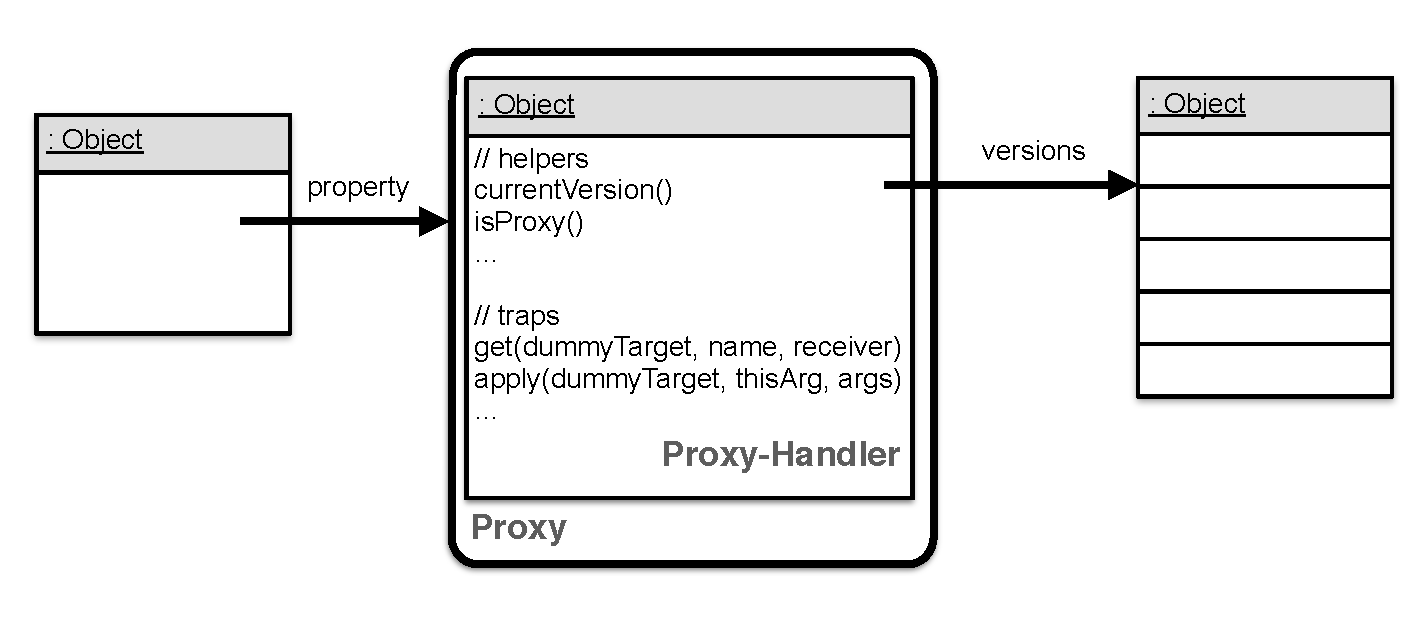
\includegraphics[width=\textwidth]{figures/5_implementation/1_versioningProxies.pdf}
    \caption{A proxy with its proxy handler, which contains traps and a reference to all versions of an object.}
    \label{fig:VersioningProxies}
\end{figure}

Each trap is provided a set of arguments to forward the access to another object.
For example, the \emph{get}-trap receives the following arguments: \lstinline{target}, \lstinline{name}, and \lstinline{receiver}.
The first of these parameters is irrelevant as it refers to a fixed target the proxy refers to, while our proxies are used as virtual objects and do not delegate to any specific object by default.
The \emph{name} parameter, however, is relevant and refers to the name of the property that was read.
The \emph{receiver} parameter is the receiving proxy and is only necessary for handling special cases.

Our proxy handler uses the traps to delegate all access to the current version of an object.
Its \emph{get}-trap is implemented as indicated by the following code snippet, which is, however, slightly simplified:

\iffalse
\begin{verbatim}\fi
\begin{code}{}{}
get: function(dummyTarget, name, receiver) {

    var version = this.currentVersion();
    
    // proxy meta information and other special cases..
    if (name === 'isProxy') {
    // ...
    if (name === 'proxyTarget') {
    // ...
    
    result = version[name];
    
    return this.ensureProxied(result);
}
\end{code}
\iffalse
\end{verbatim}\fi

First, the current version gets determined using the \lstinline{currentVersion()} helper function.
Then, multiple special cases are handled, including special properties to allow to determine whether a proxy, which otherwise behaves transparently, actually is a proxy or to unwrap the current version from the proxy.
In the case that we are only reading a property named \lstinline{age} from an object \lstinline{person} all these conditions fall through.
Instead, the trap just reads the property from the current version and returns the result.

The result is passed to the \lstinline{ensureProxied()} function to make sure that mutable objects are proxied.
When a mutable object that is not wrapped in a proxy is passed to this function, the function returns a proxy instead.
This is necessary as, while application-specific objects properties are expected to be proxied, some built-in objects in JavaScript refer to their properties directly and not through proxies, but these properties are required to be proxied as well to handle proxies correctly.

Besides the \emph{get}-trap, our proxy handler similarly provides behavior for all the other traps a Direct Proxy can have.
Table~\ref{table:traps} lists the implemented proxy traps.

\begin{table}[h]
\begin{center}
\begin{tabular}{|l|l|r|}
\hline
get: function(target, name, receiver) \\ \hline
set: function(target, name, value, receiver) \\ \hline
apply: function(target, suppliedThisArg, suppliedArgs) \\ \hline
construct: function(target, args) \\ \hline
has: function(target, name) \\ \hline
hasOwn: function(target, name) \\ \hline
defineProperty: function(target, name, desc) \\ \hline
deleteProperty: function(target, name) \\ \hline
getOwnPropertyDescriptor: function(target,name) \\ \hline
getOwnPropertyNames: function(target) \\ \hline
getPrototypeOf: function(target) \\ \hline
freeze: function(target) \\ \hline
seal: function(target) \\ \hline
preventExtensions: function(target) \\ \hline
isFrozen: function(target) \\ \hline
isSealed: function(target) \\ \hline
isExtensible: function(target) \\ \hline
enumerate: function(target) \\ \hline
keys: function(target) \\ \hline
\end{tabular}
\caption[Table caption text]{Traps implemented by our proxy handlers.}
\label{table:traps}
\end{center}
\end{table}

All these traps fire either when the proxy is accessed with specific JavaScript operators or when it is passed to meta-programming facilities provided by built-in globals\footnote{\url{http://wiki.ecmascript.org/doku.php?id=harmony:direct_proxies\#api}, accessed March 5, 2014}.
For example, the \lstinline{preventExtensions}-trap fires when a proxy is passed to the built-in \lstinline{Object.preventExtensions()} function, which prevents new properties from subsequentely being added to an object.


\subsubsection{Versions of Objects and the System}

Besides implementing the trap methods, our proxy handlers also hold the versions of the represented object.
For this, the proxy handler uses a JavaScript object to map version itentifiers to the actual versions of the object.

Having the handler object hold all the versions of conceptionally one object takes care of garbage collection.
When a proxy gets garbage collected, all versions get garbage collected as well by the normal JavaScript garbage collector.

The proxy handler chooses a \emph{version of an object} according to the global \emph{version of the system}.
A version of the system is an ordinary JavaScript object with three properties: an \lstinline{ID}, a \lstinline{previousVersion}, and a \lstinline{nextVersion}.
The current version is always referred to by \lstinline{lively.currentVersion}.
It is, therefore, globally accessible as the current version of the system.
The proxy handler uses the \lstinline{ID} of the current version to look up the version of the object.

When a version of an object is not changed in a number of versions of the system, it reflects the objects state in this group of subsequent versions.
Therefore, when a proxy traps read access, the latest version object is looked up from the dictionary of versions.
When a proxy, however, traps write access, it creates a new version of the object when no version is available for the current system version.
Creating a new version is done by shallow copying the latest available version.

For most objects, write access is trapped only in the following traps: \emph{set}, \emph{defineProperty}, \emph{deleteProperty}, \emph{preventExtension}, \emph{seal}, and \emph{freeze}.\\
Arrays, however, have built-in functions such as \lstinline{push} and \lstinline{pop} that also manipulate array state.
Therefore, the \emph{apply}-trap also checks for write access and creates new versions when necessary.

To change the entire runtime state, only the global version identifier needs to be changed.
Depending on whether the version is set to a previous version, a following version, or a new version, changing the identifier is an undo, a redo, or a commit of the current state.

Using a global version of the system is reasonable for now as JavaScript execution is single-threaded and scheduling is cooperatively in the JavaScript engines.
That is, while a JavaScript script runs, the global version cannot be changed by another script.
% At the moment, the gobal version is only changed from separate events as, for example, clicking a button that only changes the version.
% In the future, we intend to built th


% Besides this copy-on-write optimization, another optimization would be to not copy objects completely, but to only store changes.
% this could, for example, also apply prototypical inheritance to have versions that delegate to previous versions and only express the differences between versions.

\paragraph{Scope of the Versions}
Using the proxies and system versions, the state of all mutable JavaScript objects can be preserved and re-established.
Certain host objects in JavaScript engines, however, cannot be versioned.
For example, the objects that only represent the HTML elements the browser renders cannot be copied.
For this reason, when the system version changes, we update the HTML document from the current set of visible morphs.



\section{Proxies For All Mutable JavaScript Objects}

% As we use proxies as version-aware references while the JavaScript runtime still only provides ordinary references, references that usually would point to objects directly now need to point to proxies instead. 
% References to the same object need to point to the same proxy for that object as the identity of proxies will be compared instead of the identity of the original objects.
% Also, as proxies actually hold the different versions of their objects as opposed to looking the objects up in a separate data structure in our implementation, one particular proxy knows the versions of an object.
% Therefore, all references that would normally refer to the object need to refer to the proxy that stands-in for all the versions of the objects.
% To achieve this, we create proxies immediately for new objects and return the proxies instead of the objects, so a reference to the proxy gets passed around instead of the reference to the actual object, which instead is captured as a version in the versions dictionary of the proxy.
% 
% We need to create proxies for all new mutable state, which in JavaScript comprises of objects, arrays, and functions.
% Also for functions as functions are also objects and can have properties in JavaScript.
% JavaScript allows to create these kinds of objects through literal expressions, constructors, and built-in functions.
% Constructors can be built-in as, for example, \lstinline{Array} or created from literals.
% Both create new objects when applied with the \lstinline{new} keyword, but built-in constructors also return new objects when applied without the \lstinline{new} operator.
% Other built-in functions are, for example, \lstinline{eval()} or \lstinline{Object.create()}.
% To create and return proxies from all these three different ways to create objects, our implementation transforms sources before execution.
% The built-in functions could be overwritten globally to return proxies for the new objects, but our implementation of object versioning is itself just a JavaScript library and makes itself use of the built-in data types.
% Additionally, at the time of writing, some JavaScript engines do not allow to overwrite particular built-in functions and we want our implementation of object versioning to work in every JavaScript engine that supports the ECMAScript 6 Direct Proxies.
% Therefore, we transform specific literal expressions and specific built-in functions, while custom constructors return proxies through proxy trap behavior.

To have the proxies intercept access to all mutable objects, objects need to be accessed only via proxies.
This is achieved by creating proxies when objects get created and then returning references to the proxies instead of the objects.
Our implementation uses a combination of source transformations and proxy behavior to return proxies from expressions that otherwise would return new objects.
This way, programs do not have to be adapted manually to run with our implementation of object versioning.

In JavaScript, there are three different ways to create an object: 
\begin{itemize}
    \item evaluating literal expressions: e.g. \lstinline|{age: 12}|
    \item applying constructor functions: e.g. \lstinline|new Person(12)|
    \item calling specific built-in functions: e.g. \lstinline|Object.create(prototype, {age: 12})|
\end{itemize}

\paragraph{Literal Expressions}
We use source transformations to wrap literal expressions consistently into a \emph{proxyFor()} function.
That function takes an object as parameter and returns a proxy for it.
Besides objects, arrays and functions are also mutable objects in JavaScript.
Therefore, we wrap the literal forms of objects, arrays, and functions.
For exampe, \lstinline{[aPerson, aCompany]} becomes \lstinline{proxyFor([aPerson, aCompany])}.

\paragraph{Constructor Functions} 
In JavaScript, all functions can be constructors and create new objects when called with the \emph{new} operator.
Functions expressed as function literals already get proxied with the previous source transformations and the proxies we use for version-aware references intercept different object access differently, so proxies for functions can have a specific constructor-behavior that always returns proxies for newly created objects.

\paragraph{Built-in Functions}
For the built-in functions that create new objects, the transformation of literals and proxy behavior is not enough.
The main category of built-in functions are built-in constructors.
For example, the built-in data types like objects and arrays can be created by evaluating \lstinline{new Object()} and \lstinline{new Array()}, but also by evaluating just \lstinline{Object()} or \lstinline{Array()}.
We transform these built-in constructor functions explicity, wrapping each into the proxying function, and also specify the proxies' apply-behavior to also always return proxies.

Besides built-in constructors, there are also very specific built-in functions, that we transform separately to specific alternatives.
One example for such functions is the global \lstinline{eval()} function.
While the return value of that function also potentially needs to be a reference to a proxy instead of an ordinary object, eval takes arbitrary code which might express an arbitrary object structure and which might, therefore, require multiple references to go through proxies.
Therefore, in the specific case of eval, we proxy eval's result but in addition also pass the string argument of \lstinline{eval()} through the source transformations before actually providing it for evaluation.


\subsubsection{Source Transformations}

The source transformations for introducing our proxy-based version-aware references wrap the original expressions into the \lstinline{proxyFor} function, which returns a proxy for an object.
The transformations of literal objects, arrays, and functions are shown by example in Table~\ref{table:literalTransforms}.


\begin{table}[h]
\begin{center}
\begin{tabular}{| l | l | l | l |}
\hline
Type & Original code & Transformed code \\ \hline
\emph{Objects} & \lstinline|{name: 'James', age: 24}| & \lstinline|proxyFor(name: 'James', age: 24)| \\ \hline
\emph{Arrays} & \lstinline|[person1, person2]| & \lstinline|proxyFor([person1, person2])| \\ \hline
\emph{Functions} & \lstinline|function (a, b) {..}| & \lstinline|proxyFor(function (a, b) {..})| \\ \hline
\end{tabular}
\end{center}
\caption[Table caption text]{Transformations of literal objects, arrays, and functions.}
\label{table:literalTransforms}
\end{table}


Besides the straightforward wrapping of literal objects, literal arrays, and function expressions, the source transformations also needs to handle JavaScript syntax where literals cannot simply be wrapped into a function call.
Special handling is necessary for function declarations and accessor functions.

\paragraph{Function Declarations}
Function declarations are named functions, where the name is available for recursion in the function itself and also makes the function accessible by the name in the surrounding scope.
For this reason, the function declaration get transformed to function expressions that are assigned to matching variable names.
This way, \lstinline|function funcName(..) {..}| becomes \lstinline|var funcName = function funcName(..) {..}|.
In addition, because function declarations get hoisted in JavaScript, the source transformation moves the results of transforming function declarations to the beginning of the defining scope, while preserving the original order of function declarations.

\paragraph{Accessor Functions}
Accessor functions are functions that are executed instead of ordinary read or write access to properties.
The following example snippet shows the definition of a \lstinline{person} object, where two accessor functions allow reading and writing \lstinline{person.age} while the value is stored under a slightly different name:

\iffalse
\begin{verbatim}\fi
\begin{code}[lst:example]{}{float}
var person = {
    __age: 0,
    get age() {
        return this.__age;
    },
    set age(val) {
        this.__age = val;
    }
}
\end{code}
\iffalse
\end{verbatim}\fi

Wrapping the two accessor functions in-place into \lstinline{proxyFor} functions does not yield valid JavaScript code.
Therefore, the source transformations create the objects first without accessor functions and explicitly define the accessor functions using \lstinline{Object.defineProperty} later-on.
These two steps are done in an anonymous functions that is applied directly, to use a temporary variable for the newly created object to be able to refer to it in the \lstinline{Object.defineProperty}-function call, while not polluting the originally surrounding scope with an implementation-specific temporary variable.
That is, the presented example with accessor functions would be transformed to the following code: \\

\iffalse
\begin{verbatim}\fi
\begin{code}{}{}
var person = function() {
    var newObject = lively.proxyFor({
        __age: 0;
    });
    Object.defineProperty(newObject, "age", {
        get: lively.proxyFor(function age() {
            return this.__age;
        }),
        set: lively.proxyFor(function age(val) {
            this.__age = val;
        }),
        enumerable: true,
        configurable: true
    });
    return newObject;
}();'
\end{code}
\iffalse
\end{verbatim}\fi

Similar to the wrapping of object literals without accessor functions, of arrays, and of function expressions, the source transformation also wraps specific built-in functions into plain calls to the \lstinline{proxyFor()} function.
For example, \lstinline{Array(100)} becomes \lstinline{proxyFor(Array(100))}.
As every call to such built-in objects is transformed in this way, the same Object---in this case the \lstinline{Array} function---gets passed to the \lstinline{proxyFor} function multiple times.
To nevertheless return the same proxy, which also is necessary for identity checks when compared with references that go through proxies, we use a map that associates objects with their proxies.
This \emph{Proxy Table} is a weak-key map and does prevent the version object used as keys from being gargabe collected when their proxies get garbage collected.
Therefore, the following statement yields true for an arbitrary object \lstinline{obj}: \lstinline{proxyFor(obj) === proxyFor(obj)}.



\subsubsection{Returning Proxies From Proxied Constructors}

When objects get created through applying functions with the \lstinline{new} operator, the freshly created objects also need to be proxied.
However, as the functions are already proxied through source transformations of function literals and the built-in \lstinline{Function} constructor, our implementation does not transform the applications of the \lstinline{new} operator, but uses the \emph{construct} trap to return proxies from constructor applications.
The last line of code of the \lstinline{construct} function of our proxy handler is therefore: \lstinline{return this.ensureProxied(newInstance)}.
This is also true for the \emph{apply} trap, because, for example, the \lstinline{Array} and \lstinline{Object} functions also create objects when called without the \lstinline{new} operator and, for example, the built-in function \lstinline{Object.create(proto)} also returns a new object.
In fact, with our proxy handler the \emph{get}-trap also makes sure to return always proxy in this fashion.
So, wrapping \lstinline{Object} is enough to have \lstinline{Object.create(proto)} return a proxy: \lstinline{Object.create(proto)} transforms to \lstinline{proxyFor(Object).create(proto)} and getting the property \emph{create} then returns a proxy for the function, which when applied also returns a proxy.



\subsubsection{Implementation of Source Transformations}


The implementation of source transformations uses \emph{UglifyJS}\footnote{\url{http://github.com/mishoo/UglifyJS2}, accessed March 12, 2014} for parsing and for all AST transformations.
UglifyJS parses without relying on JavaScript exceptions for, for example, backtracking and, therefore, does not interfere with debugging.
In addition, UglifyJS also supports Source Maps \todo{footnote with url to Source Maps}, which allow to view and debug the original code with the browser's developer tools, even though the transformed code is executed.


\todo{add something about when the versioning source transformations are done and which parts of the system are currently versioned}
% TODO: source transformations enabled right after the object versioning code, i.e. the implementation of the proxies and the source transformation, which are both themselves implemented using ordinary javascript code, gets loaded. by patching the eval that is used for evaluated modules that get loaded with an eval(transformSource.. so modules are not versioned, but classes / layers / traits are.. e.g. a class is versioned, so in different versions there might be different class-side state... so, for example, modules are currently in our implementation the roots of the version-aware reference graphs that prevent garbage collection, 











\section{Workarounds for the Current State of the Proxies} \label{sec:IMPLEMENTATION:4}

Certain workarounds are required due to the preliminary status of the proxy implementation.

While the specification of Direct Proxies already progressed from proposal status to being part of the current ECMAScript 6 Draft\footnote{\url{http://people.mozilla.org/~jorendorff/es6-draft.html}, accessed March 5th, 2014}, it is still in draft status and not yet implemented in the JavaScript engines used by Chrome and Firefox.
These two engines currently both implement two different deprecated proposals for the proxies instead of the most recent ECMAScript 6 Draft.
The \emph{harmony-reflect} library\footnote{\url{http://github.com/tvcutsem/harmony-reflect}, accessed February 3, 2014, used version 0.0.11}, however, provides the current API of Direct Proxies for recent versions of both Chrome and Firefox, on top of the implementations of the different deprecated proposal states.
That is, our implementation uses the \emph{harmony-reflect} shim and, thereby, works in both Chrome and Firefox.

However, even with the shim, three issues need to be addressed with technical workarounds:

\begin{enumerate}
    \item The proxies have to be provided with an actual target, even when implementing virtual objects, and consistency invariants compare return values of traps to the state of the actual target. 
    \item The proxies do not intercept the \lstinline{instanceof} operator, but always delegate to the current target.
    \item Certain built-in JavaScript functions dont handle proxies correctly.
\end{enumerate}

These workarounds might no longer be necessary once the ECMAScript 6 standard gets finalized and fully implemented by the JavaScript engines. 


\subsection{Disabling Target Object Invariants}

% While these are supposed to stand-in for particular objects, their \emph{targets}, they can also be used as fully virtual objects.

Using the \emph{harmony-reflect} shim in a recent Chrome, proxies require an actual \emph{target} object even though the current ECMAScript 6 draft says otherwise\footnote{\url{http://people.mozilla.org/~jorendorff/es6-draft.html\#sec-proxy-object-internal-methods-and-internal-slots}, accessed April 15, 2014}.

When an actual target object is provided on creation of a proxy, the internal link between proxy and target object is fixed and cannot be changed at runtime.
Therefore, in our use case of the proxies, in which proxies stand-in for a group of objects from which one is chosen dynamically, the proxy is still linked to a particular object by default.
Additionally, the Direct Proxies are designed to ensure invariants between the trap behavior and the target's properties~\cite{Cutsem2013TRP}.

For example, when an object's properties are made immutable using \lstinline{Object.freeze}, the invariants ensure that the target object has in-fact been frozen, even if the trap delegates the operation to another object such as one of our versions of an object.
Further, another invariant ensures that all immutable values of the target object are returned correctly by the \lstinline{get}-trap, even when the \emph{get}-trap reads from another object than the target. 
That is, in our case, configuring any property as immutable would effectively declare make that property immutable for all versions.
Additionally, in this scenario, reading the property in a version where the value of this property is different from what it is in the immutable target would raise incosistency errors.

For this reason, we adapted our copy of the \emph{harmony-reflect} library.
In particular, we added a boolean flag to the Proxy constructor function that indicates whether a proxy is standing in for one target object or is a virtual object.
This boolean flag is then used to disable all consistency checks when a proxy is meant to be a virtual object.

The proxy constructor still requires an actual object as \emph{target} object, but this target object is now only used for the \lstinline{typeof} operator for the virtual object-kind of proxies.

The \lstinline{typeof} operator returns only a distinction between a certain set of types in JavaScript.
The only necessary difference for the \lstinline{typeof} operator is that a proxy representing the versions of an object or array has an object as target, while a proxy representing the versions of a function needs to have a function as target.
This difference in the type of supplied target objects is also necessary as the \emph{apply}- and \emph{construct}-trap are also only called on proxies with functions as targets.


\subsection{Forwarding the \emph{Instanceof} Operator}

There is currently no \lstinline{instanceof} trap to intercept the behavior of the \lstinline{instanceof} operator.

The \lstinline{instanceof} operator returns the of an object, which is defined by an object's prototype chain in JavaScript.
The prototype of an object is a property and can be changed at runtime.
It gets versioned as any other property.
The \lstinline{instanceof} operator, thus, also needs to be delegated to the current version of an object.
% When creating a proxy a \emph{target} object can be provided to be linked from the proxy and the \lstinline{instanceof} operator would follow this link to report the target's type, but as the target link cannot be changed later on, while proxies stand-in for multiple versions with potentially different types, this is not an option.

For this, we implemented a custom \lstinline{Object.instanceof()} function, which implements the semantics of the \lstinline{instanceof} operator but does delegate to the correct version of an object.
All usage of the \lstinline{instanceof} operator is then transformed to usage of the custom function.
These transformations change code as shown by the following example: 

\iffalse
\begin{verbatim}\fi
\begin{code}[]{}{float}
anObject instanceof Type -> Object.instanceof(anObject, Type)
\end{code}
\iffalse
\end{verbatim}\fi

While there is no trap for the \lstinline{instanceof} operator in the current specification, trapping the operator is under discussion\footnote{\url{http://wiki.ecmascript.org/doku.php?id=harmony:direct_proxies\#discussed_during_tc39_july_2012_meeting_microsoft_redmond}, accessed May 1, 2014}.


\subsection{Unwrapping Versions for Native Code}

Some built-in JavaScript functions react to proxies with actual errors, return wrong results, or otherwise do not provide the usual functionality.
Therefore, these functions need to be provided with actual objects instead of the proxy.
% This is unproblematic for most cases as, given JavaScript's single-threaded and cooperative execution in browser engines, which version of an object is to be used is not expected to change during the execution of a built-in function.
Our implementation provides the current version of an object to these built-in functions through proxy handler traps and patched built-in functions.

The \emph{apply}-trap, called when proxied functions get applied, unwraps all arguments and the \emph{thisContext} object, when the applied function is a built-in functions that does not handle proxies correctly.
This is for example the case for the functions that provide access to the browser's document model.

The \emph{set}-trap sometimes needs to unwrap the assigned value when that value is proxied and gets assigned to slots that cannot handle proxies.
This is for example the case with the \lstinline{onreadystatechange} slot of \emph{XMLHttpRequest} objects.
This particular slot holds functions as callbacks of asynchronous HTTP requests, which, however, do not get called when these functions are proxies.

The unwrapping a particular version from a proxy for an asynchronous callback is potentially problematic.
Though JavaScript does get executed with a single thread using cooperative scheduling by all popular browsers, other concurrent scripts might get executed and switch the global version before the callback can be called.
It is, however, unlikely that a callback function's \emph{properties} are changed while waiting for the response and even bad programming style as it introduces dependencies on network timing even without proxies.
Therefore, our implementation currently does not provide a workaround for this specific case, even though we are aware of this potential problem. 

In addition to unwrapping in traps, there are also certain immutable types that do not get proxied at all in our implemention such as strings.
Strings, however, do have methods and these also do not handle proxies correctly.
As the arguments to these methods is not handled in traps, because strings are not proxied, our implementation patches such functions with functions that unwrap proxies before executing the original functions.









\section{Limitations of the Implementation}

\todosec{write this section from the following notes}

% content: limitations of our implementation that are not directly related to the state of the preliminary implementation of the proxies.. except for the general limitation that these proxies have to be available, e.g. experimental javascript enabled in chrome

our implementation is based on and requires the ECMAScript 6 Direct Proxies to be available.
however, as these are at the moment only part of the next draft of ECMAScript and not yet finalized, the implementation only works when the nevertheless are available, which is currently.. recent versions of Chrome with experimental JavaScript explicitly enabled and in recent versions of Firefox


% TODO: Limitations for Concurrent JavaScript

single-threaded and cooperative scheduling, but setTimeout / setInterval... stop asynchronous actions from following versions when undoing... source transformations, which scripts belongs to which version



% TODO: Usability: Impact on Debugging

adds lots of low-level frames due to the partly native but also partly shim implementation of proxies..

dev tools don’t yet handle proxies well (hovering, labels, stepping into), but we have at least source maps, so developers can debug the original code and not the result of our source transformation
Besides impacting code execution, the current implementation of object versioning for the Lively Kernel also with certain programming tasks.
Though the version-aware references should be transparent to programmers, in the current proxy-based implementation proxies show during debugging.
However, the developer tools show the original source code, despite the implementation's transformations of the sources.





% Nevertheless, our implementation is functional and integrated with the Lively Kernel.
% It allows programmers to undo and redo changes and is publicly available\footnote{\url{http://github.com/LivelyKernel/LivelyKernel/commit/858aca8c5ac0f203061823f463fda9b434131636}}.
